\section{Meltdown-Spectre Attacks}
\subsection{Meltdown}
\subsubsection{Basics}
Architectural state $\not = $ Microarchitectural state

Cache location depends on actual data address.

\begin{description}
    \item[Page tables] translate virt. address to physical address
    \item[Page table entry (PTE)] includes permission bits and who is allowed to access
    \item[Pipelining] split instruction into
        \begin{itemize}
            \item instr. fetch (IF)
            \item instr. decode (ID)
            \item execute (EX)
            \item memory access (MEM)
            \item write back (WB)
        \end{itemize}
    \item[Out-of-Order execution] parallelize execute stage (EX). Run all instr. without inter dependencies in parallel. Retire in-order.
\end{description}


\subsubsection{Attack}
Idea: Microarchitectural state (caches) is modified even if memory access was not allowed.

\begin{center}
    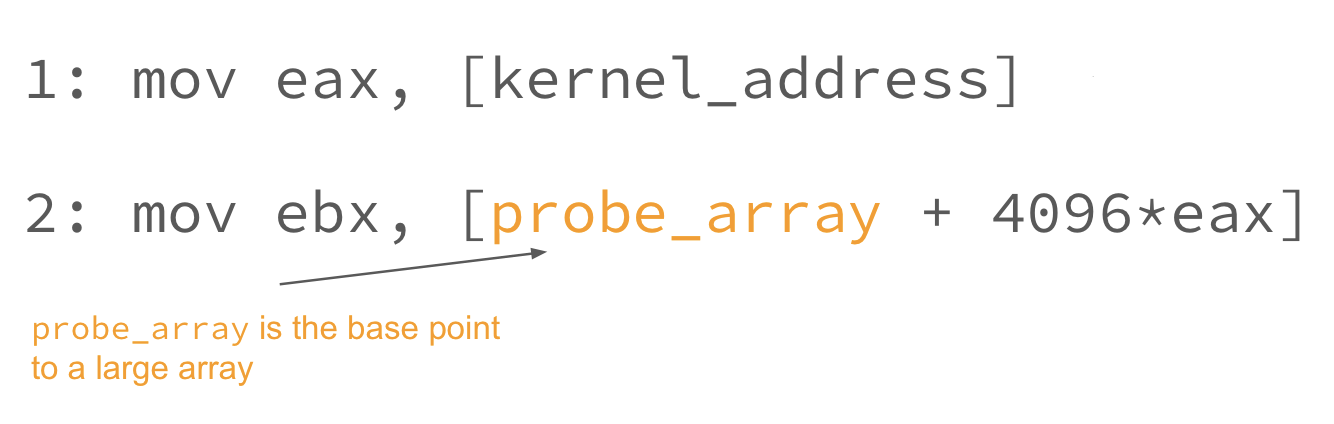
\includegraphics[width=0.8\linewidth]{images/meltdown-cache.png}
\end{center}

\texttt{probe\char`_array} will be accessed at an index which depends on the
secret (e.g. data in kernel address space $[$\texttt{kernel\char`_address}$]$).
Check cache load times for all indices of array to get the index which was accessed by prohibited memory read.

\subsection{Spectre}
\begin{itemize}
    \item based on branch prediction and speculative execution
    \item dynamic predictors use runtime information
    \item Branch Target Buffer (BTB) does not store information about process id or virt. address it belongs to $\xrightarrow{}$ same for each core $\xrightarrow{}$ can be trained by process A but used for B
\end{itemize}

\subsubsection{Spectre 1}
Attacker has control over input used in branch (here \texttt{x}).

\textbf{Can only read memory accessible for process,} but not to the attacker (no privileged read).

\begin{center}
    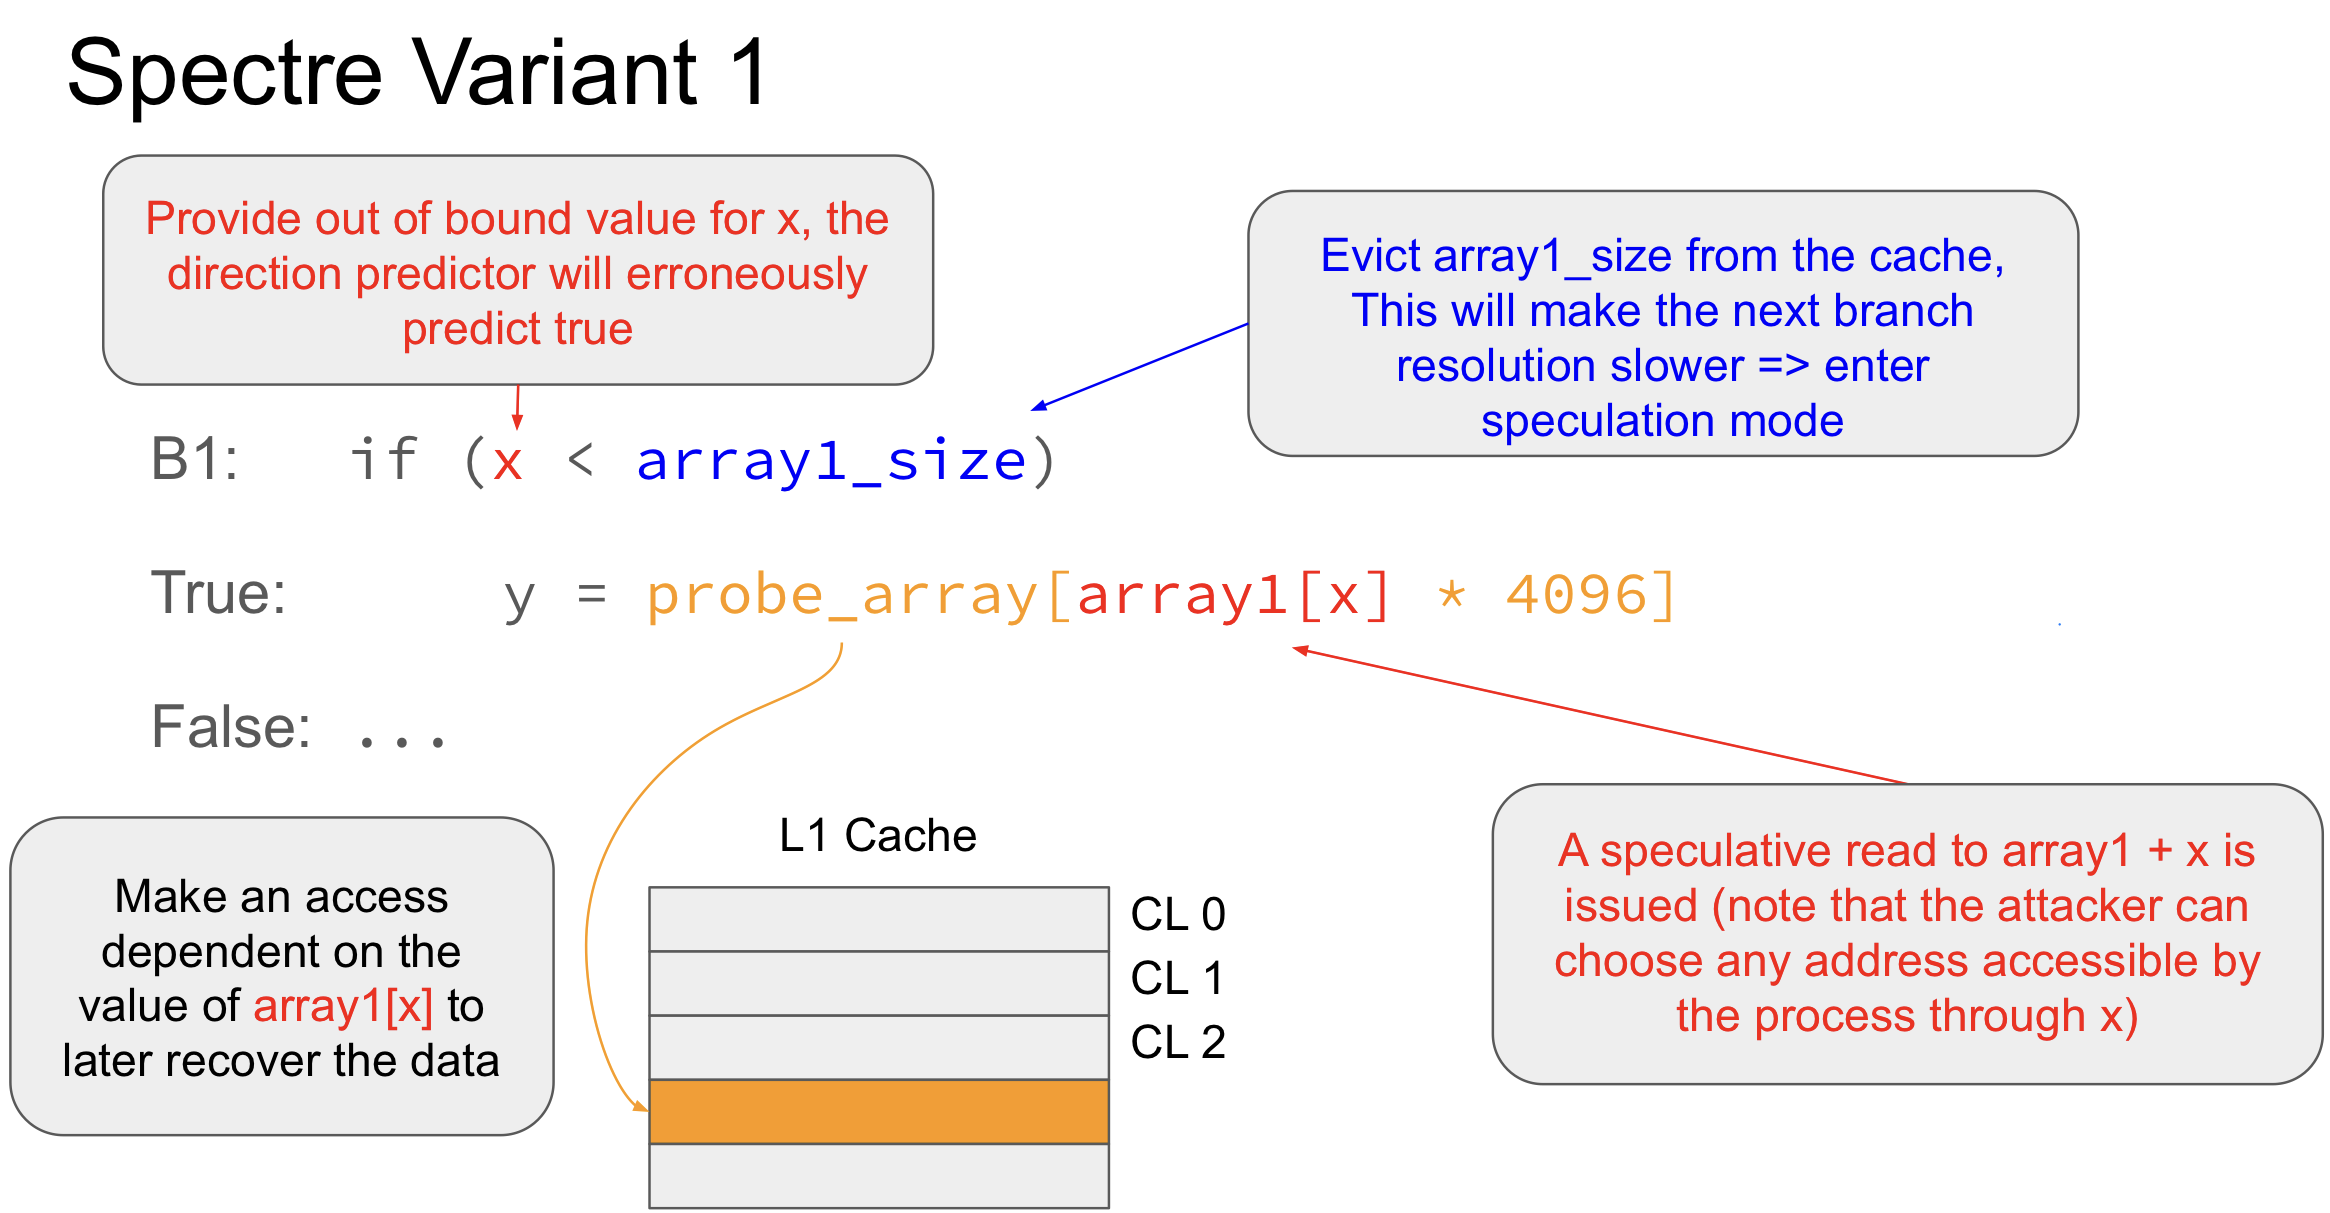
\includegraphics[width=\linewidth]{images/spectre1-overview.png}
\end{center}

\subsubsection{Spectre 2}
Idea: Mistrain BTB to exec. code which creates a side-channel $\xrightarrow{}$
spectre gadget.\\
Unlike Meltdown this does not exploit race condition.

Gadget should:\vspace{-1.5mm}
\begin{enumerate}
    \item exec memory access controlled by attacker's input
    \item exec instr which creates change in microarchitectural state
\end{enumerate}

Attacker needs:\vspace{-1.5mm}
\begin{itemize}
    \item 1 input to select memory location to read
    \item 1 input to control how to leak (e.g. base pointer of \texttt{probe\char`_array})
\end{itemize}
